% Options for packages loaded elsewhere
% Options for packages loaded elsewhere
\PassOptionsToPackage{unicode}{hyperref}
\PassOptionsToPackage{hyphens}{url}
\PassOptionsToPackage{dvipsnames,svgnames,x11names}{xcolor}
%
\documentclass[
  french,
  10pt,
  a4paper,
]{article}
\usepackage{xcolor}
\usepackage[top=20mm,left=20mm,right=20mm,bottom=20mm]{geometry}
\usepackage{amsmath,amssymb}
\setcounter{secnumdepth}{5}
\usepackage{iftex}
\ifPDFTeX
  \usepackage[T1]{fontenc}
  \usepackage[utf8]{inputenc}
  \usepackage{textcomp} % provide euro and other symbols
\else % if luatex or xetex
  \usepackage{unicode-math} % this also loads fontspec
  \defaultfontfeatures{Scale=MatchLowercase}
  \defaultfontfeatures[\rmfamily]{Ligatures=TeX,Scale=1}
\fi
\usepackage{lmodern}
\ifPDFTeX\else
  % xetex/luatex font selection
  \setmainfont[]{Raleway}
  \setsansfont[]{Avenir Next LT Pro}
  \setmonofont[Scale=0.9]{Consolas}
\fi
% Use upquote if available, for straight quotes in verbatim environments
\IfFileExists{upquote.sty}{\usepackage{upquote}}{}
\IfFileExists{microtype.sty}{% use microtype if available
  \usepackage[]{microtype}
  \UseMicrotypeSet[protrusion]{basicmath} % disable protrusion for tt fonts
}{}
\makeatletter
\@ifundefined{KOMAClassName}{% if non-KOMA class
  \IfFileExists{parskip.sty}{%
    \usepackage{parskip}
  }{% else
    \setlength{\parindent}{0pt}
    \setlength{\parskip}{6pt plus 2pt minus 1pt}}
}{% if KOMA class
  \KOMAoptions{parskip=half}}
\makeatother
% Make \paragraph and \subparagraph free-standing
\makeatletter
\ifx\paragraph\undefined\else
  \let\oldparagraph\paragraph
  \renewcommand{\paragraph}{
    \@ifstar
      \xxxParagraphStar
      \xxxParagraphNoStar
  }
  \newcommand{\xxxParagraphStar}[1]{\oldparagraph*{#1}\mbox{}}
  \newcommand{\xxxParagraphNoStar}[1]{\oldparagraph{#1}\mbox{}}
\fi
\ifx\subparagraph\undefined\else
  \let\oldsubparagraph\subparagraph
  \renewcommand{\subparagraph}{
    \@ifstar
      \xxxSubParagraphStar
      \xxxSubParagraphNoStar
  }
  \newcommand{\xxxSubParagraphStar}[1]{\oldsubparagraph*{#1}\mbox{}}
  \newcommand{\xxxSubParagraphNoStar}[1]{\oldsubparagraph{#1}\mbox{}}
\fi
\makeatother

\usepackage{color}
\usepackage{fancyvrb}
\newcommand{\VerbBar}{|}
\newcommand{\VERB}{\Verb[commandchars=\\\{\}]}
\DefineVerbatimEnvironment{Highlighting}{Verbatim}{commandchars=\\\{\}}
% Add ',fontsize=\small' for more characters per line
\newenvironment{Shaded}{}{}
\newcommand{\AlertTok}[1]{\textcolor[rgb]{0.58,0.85,0.30}{\textbf{\colorbox[rgb]{0.30,0.12,0.14}{#1}}}}
\newcommand{\AnnotationTok}[1]{\textcolor[rgb]{0.31,0.63,0.31}{#1}}
\newcommand{\AttributeTok}[1]{\textcolor[rgb]{0.65,0.15,0.64}{#1}}
\newcommand{\BaseNTok}[1]{\textcolor[rgb]{0.60,0.41,0.00}{#1}}
\newcommand{\BuiltInTok}[1]{\textcolor[rgb]{0.65,0.15,0.64}{#1}}
\newcommand{\CharTok}[1]{\textcolor[rgb]{0.31,0.63,0.31}{#1}}
\newcommand{\CommentTok}[1]{\textcolor[rgb]{0.63,0.63,0.65}{\textit{#1}}}
\newcommand{\CommentVarTok}[1]{\textcolor[rgb]{0.89,0.34,0.29}{\textit{#1}}}
\newcommand{\ConstantTok}[1]{\textcolor[rgb]{0.60,0.41,0.00}{#1}}
\newcommand{\ControlFlowTok}[1]{\textcolor[rgb]{0.65,0.15,0.64}{#1}}
\newcommand{\DataTypeTok}[1]{\textcolor[rgb]{0.65,0.15,0.64}{#1}}
\newcommand{\DecValTok}[1]{\textcolor[rgb]{0.60,0.41,0.00}{#1}}
\newcommand{\DocumentationTok}[1]{\textcolor[rgb]{0.89,0.34,0.29}{#1}}
\newcommand{\ErrorTok}[1]{\textcolor[rgb]{0.96,0.28,0.28}{\underline{#1}}}
\newcommand{\ExtensionTok}[1]{\textcolor[rgb]{0.25,0.47,0.95}{\textbf{#1}}}
\newcommand{\FloatTok}[1]{\textcolor[rgb]{0.60,0.41,0.00}{#1}}
\newcommand{\FunctionTok}[1]{\textcolor[rgb]{0.25,0.47,0.95}{#1}}
\newcommand{\ImportTok}[1]{\textcolor[rgb]{0.31,0.63,0.31}{#1}}
\newcommand{\InformationTok}[1]{\textcolor[rgb]{0.77,0.36,0.00}{#1}}
\newcommand{\KeywordTok}[1]{\textcolor[rgb]{0.65,0.15,0.64}{#1}}
\newcommand{\NormalTok}[1]{\textcolor[rgb]{0.22,0.23,0.26}{#1}}
\newcommand{\OperatorTok}[1]{\textcolor[rgb]{0.65,0.15,0.64}{#1}}
\newcommand{\OtherTok}[1]{\textcolor[rgb]{0.15,0.68,0.38}{#1}}
\newcommand{\PreprocessorTok}[1]{\textcolor[rgb]{0.65,0.15,0.64}{#1}}
\newcommand{\RegionMarkerTok}[1]{\textcolor[rgb]{0.16,0.50,0.73}{\colorbox[rgb]{0.08,0.19,0.26}{#1}}}
\newcommand{\SpecialCharTok}[1]{\textcolor[rgb]{0.00,0.52,0.74}{#1}}
\newcommand{\SpecialStringTok}[1]{\textcolor[rgb]{0.85,0.27,0.33}{#1}}
\newcommand{\StringTok}[1]{\textcolor[rgb]{0.31,0.63,0.31}{#1}}
\newcommand{\VariableTok}[1]{\textcolor[rgb]{0.89,0.34,0.29}{#1}}
\newcommand{\VerbatimStringTok}[1]{\textcolor[rgb]{0.85,0.27,0.33}{#1}}
\newcommand{\WarningTok}[1]{\textcolor[rgb]{0.85,0.27,0.33}{#1}}

\usepackage{longtable,booktabs,array}
\newcounter{none} % for unnumbered tables
\usepackage{calc} % for calculating minipage widths
% Correct order of tables after \paragraph or \subparagraph
\usepackage{etoolbox}
\makeatletter
\patchcmd\longtable{\par}{\if@noskipsec\mbox{}\fi\par}{}{}
\makeatother
% Allow footnotes in longtable head/foot
\IfFileExists{footnotehyper.sty}{\usepackage{footnotehyper}}{\usepackage{footnote}}
\makesavenoteenv{longtable}
\usepackage{graphicx}
\makeatletter
\newsavebox\pandoc@box
\newcommand*\pandocbounded[1]{% scales image to fit in text height/width
  \sbox\pandoc@box{#1}%
  \Gscale@div\@tempa{\textheight}{\dimexpr\ht\pandoc@box+\dp\pandoc@box\relax}%
  \Gscale@div\@tempb{\linewidth}{\wd\pandoc@box}%
  \ifdim\@tempb\p@<\@tempa\p@\let\@tempa\@tempb\fi% select the smaller of both
  \ifdim\@tempa\p@<\p@\scalebox{\@tempa}{\usebox\pandoc@box}%
  \else\usebox{\pandoc@box}%
  \fi%
}
% Set default figure placement to htbp
\def\fps@figure{htbp}
\makeatother



\ifLuaTeX
\usepackage[bidi=basic,shorthands=off]{babel}
\else
\usepackage[bidi=default,shorthands=off]{babel}
\fi
\ifPDFTeX
\else
\babelfont{rm}[]{Raleway}
\fi
\ifLuaTeX
  \usepackage{selnolig} % disable illegal ligatures
\fi


\setlength{\emergencystretch}{3em} % prevent overfull lines

\providecommand{\tightlist}{%
  \setlength{\itemsep}{0pt}\setlength{\parskip}{0pt}}



 


\usepackage{booktabs}
\usepackage{longtable}
\usepackage{array}
\usepackage{multirow}
\usepackage{wrapfig}
\usepackage{float}
\usepackage{colortbl}
\usepackage{pdflscape}
\usepackage{tabularx}
\usepackage{xltabular}
\usepackage{threeparttable}
\usepackage{threeparttablex}
\usepackage[normalem]{ulem}
\usepackage{makecell}
\usepackage{xcolor}
% Retour à la ligne du texte pour qu'il ne dépasse pas dans les marges du document
\usepackage{fvextra}
\DefineVerbatimEnvironment{Highlighting}{Verbatim}{breaklines,breakanywhere,commandchars=\\\{\}}
\renewenvironment{verbatim}{\VerbatimEnvironment\begin{Verbatim}[breaklines=true,breakanywhere=true]}{\end{Verbatim}}


\usepackage{graphicx} % pour insérer des images
\usepackage{fancyhdr} % gestion du header / footer
\pagestyle{plain}     % style par défaut avec numéro de page centré en bas

% STYLE « firstpage » : pied de page personnalisé pour la première page
\fancypagestyle{firstpage}{
  % vide header et footer
  \fancyhf{} % 
  % --- suppression des lignes horizontales ---
  \renewcommand{\headrulewidth}{0pt} % supprime la ligne horizontale de l'en-tête
  \renewcommand{\footrulewidth}{0pt} % supprime la ligne horizontale du pied de page
  % --- ajustement local de la distance du bas = augmenter \footskip localement avec \setlength ---
  \setlength{\footskip}{1pt}
  %  --- contenu du pied de page centré ---
  \fancyfoot[C]{%
    Diffusé sous licence CC BY-NC-SA 4.0 \\[6pt] % texte avec saut de ligne vertical
    
\includegraphics[height=1cm]{img/Licence_cc-by-nc-sa.png} \\[10pt] % logo en dessous puis ligne vide supplémentaire
    }
    }
\makeatletter
\@ifpackageloaded{tcolorbox}{}{\usepackage[skins,breakable]{tcolorbox}}
\@ifpackageloaded{fontawesome5}{}{\usepackage{fontawesome5}}
\definecolor{quarto-callout-color}{HTML}{909090}
\definecolor{quarto-callout-note-color}{HTML}{0758E5}
\definecolor{quarto-callout-important-color}{HTML}{CC1914}
\definecolor{quarto-callout-warning-color}{HTML}{EB9113}
\definecolor{quarto-callout-tip-color}{HTML}{00A047}
\definecolor{quarto-callout-caution-color}{HTML}{FC5300}
\definecolor{quarto-callout-color-frame}{HTML}{acacac}
\definecolor{quarto-callout-note-color-frame}{HTML}{4582ec}
\definecolor{quarto-callout-important-color-frame}{HTML}{d9534f}
\definecolor{quarto-callout-warning-color-frame}{HTML}{f0ad4e}
\definecolor{quarto-callout-tip-color-frame}{HTML}{02b875}
\definecolor{quarto-callout-caution-color-frame}{HTML}{fd7e14}
\makeatother
\makeatletter
\@ifpackageloaded{caption}{}{\usepackage{caption}}
\AtBeginDocument{%
\ifdefined\contentsname
  \renewcommand*\contentsname{Table des matières}
\else
  \newcommand\contentsname{Table des matières}
\fi
\ifdefined\listfigurename
  \renewcommand*\listfigurename{Liste des Figures}
\else
  \newcommand\listfigurename{Liste des Figures}
\fi
\ifdefined\listtablename
  \renewcommand*\listtablename{Liste des Tables}
\else
  \newcommand\listtablename{Liste des Tables}
\fi
\ifdefined\figurename
  \renewcommand*\figurename{Figure}
\else
  \newcommand\figurename{Figure}
\fi
\ifdefined\tablename
  \renewcommand*\tablename{Tableau}
\else
  \newcommand\tablename{Tableau}
\fi
}
\@ifpackageloaded{float}{}{\usepackage{float}}
\floatstyle{ruled}
\@ifundefined{c@chapter}{\newfloat{codelisting}{h}{lop}}{\newfloat{codelisting}{h}{lop}[chapter]}
\floatname{codelisting}{Listing}
\newcommand*\listoflistings{\listof{codelisting}{Liste des Listings}}
\captionsetup{labelsep=period}
\makeatother
\makeatletter
\makeatother
\makeatletter
\@ifpackageloaded{caption}{}{\usepackage{caption}}
\@ifpackageloaded{subcaption}{}{\usepackage{subcaption}}
\makeatother
\makeatletter
\@ifpackageloaded{tcolorbox}{}{\usepackage[skins,breakable]{tcolorbox}}
\makeatother
\makeatletter
\@ifundefined{shadecolor}{\definecolor{shadecolor}{rgb}{.97, .97, .97}}{}
\makeatother
\makeatletter
\makeatother
\makeatletter
\ifdefined\Shaded\renewenvironment{Shaded}{\begin{tcolorbox}[borderline west={3pt}{0pt}{shadecolor}, boxrule=0pt, breakable, enhanced, frame hidden, interior hidden, sharp corners]}{\end{tcolorbox}}\fi
\makeatother
\usepackage{bookmark}
\IfFileExists{xurl.sty}{\usepackage{xurl}}{} % add URL line breaks if available
\urlstyle{same}
% fallback for those not using the hyperref driver hyperxmp:
\makeatletter
\@ifundefined{xmpquote}{\newcommand{\xmpquote}[1]{#1}}{}
\makeatother
\hypersetup{
  pdftitle={Bulle d'R. (Re)Découvrir Quarto sous R},
  pdfauthor={Sandrine LYSER},
  pdflang={fr},
  colorlinks=true,
  linkcolor={blue},
  filecolor={Maroon},
  citecolor={Blue},
  urlcolor={Blue},
  pdfcreator={LaTeX via pandoc}}


\title{Bulle d'R. (Re)Découvrir Quarto sous R}
\author{Sandrine LYSER}
\date{15 octobre 2026}
\begin{document}
\maketitle

\renewcommand*\contentsname{Table des matières}
{
\setcounter{tocdepth}{3}
\tableofcontents
}

\thispagestyle{firstpage}
\pagebreak

\section*{}\label{section}

\subsection*{Jeu de données utilisé dans cette
session}\label{jeu-de-donnuxe9es-utilisuxe9-dans-cette-session}
\addcontentsline{toc}{subsection}{Jeu de données utilisé dans cette
session}

\textbf{\texttt{hdv2003}}

\begin{itemize}
\tightlist
\item
  disponible dans le package
  \href{https://juba.github.io/questionr/index.html}{\texttt{\{questionr\}}}
\item
  échantillon tiré de l'enquête Histoire de vie, réalisée en 2003 en
  France, par l'Insee, auprès de la population âgée de 18 ans et plus
\item
  2000 lignes et 20 variables
\end{itemize}

\textbf{Dictionnaire des variables}

\begin{longtable*}[t]{lll}
\toprule
Variable & Description & Type\\
\midrule
id & Identifiant unique de l'individu & entier\\
age & Âge de l'individu & entier\\
sexe & Sexe de l'individu & facteur (Femme, Homme)\\
nivetud & Niveau d'études & facteur (8 modalités)\\
poids & Poids de l'individu dans l'échantillon & numérique\\
\addlinespace
occup & Occupation principale & facteur (7 modalités)\\
qualif & Qualification professionnelle & facteur (7 modalités)\\
freres.soeurs & Nombre de frères et soeurs & entier\\
clso & Classe sociale & facteur (3 modalités)\\
relig & Religion & facteur (6 modalités)\\
\addlinespace
trav.imp & Importance accordée au travail & facteur (4 modalités)\\
trav.satisf & Satisfaction au travail & facteur (3 modalités)\\
hard.rock & Écoute du hard rock & facteur (Oui, Non)\\
lecture.bd & Lecture de bandes dessinées & facteur (Oui, Non)\\
peche.chasse & Pratique de la pêche ou de la chasse & facteur (Oui, Non)\\
\addlinespace
cuisine & Pratique de la cuisine & facteur (Oui, Non)\\
bricol & Pratique du bricolage & facteur (Oui, Non)\\
cinema & Fréquentation du cinéma & facteur (Oui, Non)\\
sport & Pratique d'un sport & facteur (Oui, Non)\\
heures.tv & Nombre d'heures passées devant la télévision & numérique\\
\bottomrule
\end{longtable*}

\section{Introduction générale}\label{introduction-guxe9nuxe9rale}

\subsection{Le problème de
départ\ldots{}}\label{le-probluxe8me-de-duxe9part}

Une étude contient

\begin{itemize}
\tightlist
\item
  le code qui transforme les données\\
\item
  les tableaux et graphiques produits\\
\item
  le texte qui explique les résultats\\
\item
  le rapport ou la présentation à partager
\end{itemize}


\includegraphics[width=1em,height=1em]{index_files/figure-pdf/fa-icon-09adc4e6f7e3a3ea6746cbc6d7cc075a.pdf}
\textbf{Quand ces éléments sont séparés, il faut les mettre à jour
manuellement et vérifier qu'ils racontent toujours la même histoire}

\subsection{Les questions
associées\ldots{}}\label{les-questions-associuxe9es}

\begin{itemize}
\tightlist
\item
  Comment éviter les copier-coller des résultats pour que le document
  Word corresponde bien aux résultats ?\\
\item
  Comment rendre son travail intelligible pour les collègues (et
  soi-même) ?\\
\item
  Comment assurer une certaine reproductibilité du travail ?\\
\item
  Comment mettre à disposition du code ?
\end{itemize}


\includegraphics[width=1em,height=1em]{index_files/figure-pdf/fa-icon-a978eb57bd05d19791fd4e4b9d979961.pdf}
\textbf{Il existe des outils pour résoudre ces problèmes liés au partage
et la reproductibilité du travail}

\subsection{La programmation lettrée}\label{la-programmation-lettruxe9e}

\textbf{Idée centrale :} associer dans un même document du code, des
explications et des résultats

\begin{Shaded}
\begin{Highlighting}[]
\NormalTok{Ce script est dédié aux premières analyses des données hdv2003 du package "questionr"}

\FunctionTok{\#  Étape 1. Chargement des packages}
\NormalTok{Dans un premier temps on charge les packages R}
\NormalTok{  \textasciigrave{}\{r\}}
\NormalTok{  \# Packages}
\NormalTok{  library(tidyverse)  \# v2.0.0}
\NormalTok{  library(questionr)  \# v0.8.2}
\NormalTok{  \textasciigrave{}}

\FunctionTok{\#  Étape 2. Chargement des données}
\NormalTok{Dans un second temps on charge les données}
\NormalTok{  \textasciigrave{}\{r\}}
\NormalTok{  \# Chargement des données depuis le package "questionr"}
\NormalTok{  data(hdv2003)}
\NormalTok{  \textasciigrave{}}

\FunctionTok{\#  Étape 3. Analyses}
\FunctionTok{\#\# Tableau}
\NormalTok{Puis on crée un premier tableau qui montre la distribution de la variable sexe}
\NormalTok{  \textasciigrave{}\{r\}}
\NormalTok{  hdv2003 |\textgreater{} }
\NormalTok{    select(sexe) |\textgreater{} }
\NormalTok{    questionr::freq(total = TRUE)}
\NormalTok{  \textasciigrave{}}

\FunctionTok{\#\# Graphique}
\NormalTok{Enfin, on crée un graphique, qui illustre la différence du nombre d\textquotesingle{}heures passées devant la télévision selon le sexe}
\NormalTok{  \textasciigrave{}\{r\}}
\NormalTok{  hdv2003 |\textgreater{} }
\NormalTok{  ggplot() +}
\NormalTok{    aes(heures.tv) + }
\NormalTok{    geom\_boxplot() + }
\NormalTok{    facet\_wrap(vars(sexe))}
\NormalTok{  \textasciigrave{}}
\end{Highlighting}
\end{Shaded}

\begin{itemize}
\tightlist
\item
  Le texte explique \textbf{pourquoi} et \textbf{comment} l'analyse est
  réalisée\\
\item
  Le code est exécuté lors du rendu (\texttt{Render})\\
\item
  Les sorties, tableaux et graphiques sont insérés automatiquement dans
  le document final\\
\item
  Le document reste lisible sans être un simple script commenté\\
\item
  Modifier les données ou le code peut mettre à jour tout le document
\end{itemize}

\subsection{\texorpdfstring{Programmation classique \emph{vs}
programmation
lettrée}{Programmation classique vs programmation lettrée}}\label{programmation-classique-vs-programmation-lettruxe9e}

{\def\LTcaptype{none} % do not increment counter
\begin{longtable}[]{@{}
  >{\raggedright\arraybackslash}p{(\linewidth - 4\tabcolsep) * \real{0.3571}}
  >{\raggedright\arraybackslash}p{(\linewidth - 4\tabcolsep) * \real{0.3214}}
  >{\raggedright\arraybackslash}p{(\linewidth - 4\tabcolsep) * \real{0.3214}}@{}}
\toprule\noalign{}
\begin{minipage}[b]{\linewidth}\raggedright
\end{minipage} & \begin{minipage}[b]{\linewidth}\raggedright
Programmation classique
\end{minipage} & \begin{minipage}[b]{\linewidth}\raggedright
Programmation lettrée
\end{minipage} \\
\midrule\noalign{}
\endhead
\bottomrule\noalign{}
\endlastfoot
Type de fichier & .R & .rmd, .qmd \\
Organisation des fichiers & Script et rapport séparés & Code et analyse
regroupés \\
Contenu du fichier & Code prédominant & Texte prédominant \\
Documentation & Brefs commentaires & Texte explicatif détaillé \\
Lecture & Orientée code & Orientée documentation \\
Intégration des résultats & Par copier-coller & Grâce à la
compilation \\
Mise à jour des tables/plots & Manuelle & Lors de la compilation \\
Reproductibilité & Limitée & Facilitée \\
\end{longtable}
}


\includegraphics[width=1em,height=1em]{index_files/figure-pdf/fa-icon-a978eb57bd05d19791fd4e4b9d979961.pdf}
\textbf{Quarto applique ce principe de programmation lettrée}

\section{Présentation de Quarto}\label{pruxe9sentation-de-quarto}

\subsection{Quarto en une idée}\label{quarto-en-une-iduxe9e}

\begin{center}
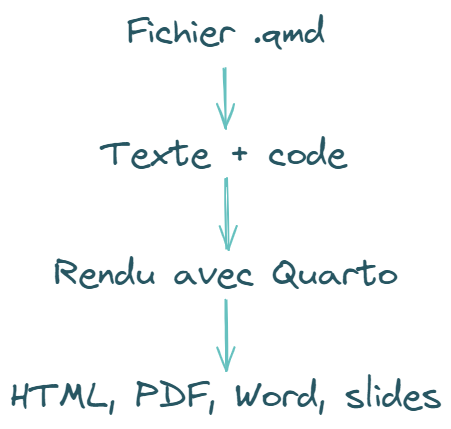
\includegraphics[width=0.6\linewidth,height=\textheight,keepaspectratio]{img/quarto_workflow_20261012.png}
\end{center}

Un seul fichier qui rassemble

\begin{itemize}
\tightlist
\item
  du texte rédigé en \textbf{Markdown}\\
\item
  du code \textbf{R} et/ou dans d'autres langages
\item
  les résultats produits par ce code
\end{itemize}

et qui est compilé pour générer un document, un site ou une présentation


\includegraphics[width=1em,height=1em]{index_files/figure-pdf/fa-icon-a978eb57bd05d19791fd4e4b9d979961.pdf}
\textbf{Le fichier source au format \texttt{.qmd} est modifiable}\\

\includegraphics[width=1em,height=1em]{index_files/figure-pdf/fa-icon-a978eb57bd05d19791fd4e4b9d979961.pdf}
\textbf{Le rendu, qui peut prendre plusieurs formats de sortie, est le
résultat prêt à être diffusé et partagé}

\subsection{Utiliser Quarto dans
RStudio}\label{utiliser-quarto-dans-rstudio}

\subsubsection{1. Installer les outils}\label{installer-les-outils}

\begin{itemize}
\tightlist
\item
  Installer \href{https://cran.r-project.org/}{\textbf{R}}\\
\item
  Installer
  \href{https://posit.co/download/rstudio-desktop/}{\textbf{RStudio}}\\
\item
  Installer l'extension \textbf{Quarto} dans \textbf{RStudio} si
  nécessaire
\end{itemize}


\includegraphics[width=1em,height=1em]{index_files/figure-pdf/fa-icon-a62d11e1500f8a927ee7cb35ace101f4.pdf}
\textbf{RStudio} propose une interface intégrée pour créer, modifier et
compiler des documents \textbf{Quarto}

\begin{center}\rule{0.5\linewidth}{0.5pt}\end{center}

\subsubsection{2. Créer un document}\label{cruxe9er-un-document}

Dans \textbf{RStudio}

\begin{enumerate}
\def\labelenumi{\arabic{enumi}.}
\tightlist
\item
  \textbf{File} → \textbf{New File} → \textbf{Quarto Document\ldots{}}\\
\item
  Choisir un titre, un auteur ou une autrice, et éventuellement le
  format de sortie\\
\item
  Choisir \textbf{html}, \textbf{pdf}, \textbf{Word} ou une
  présentation\\
\item
  Cliquer sur \textbf{Create}\\
\end{enumerate}


\includegraphics[width=1em,height=1em]{index_files/figure-pdf/fa-icon-a978eb57bd05d19791fd4e4b9d979961.pdf}
\textbf{RStudio} crée un fichier \texttt{.qmd} contenant déjà un YAML,
du texte et un exemple de bloc de code

\begin{center}
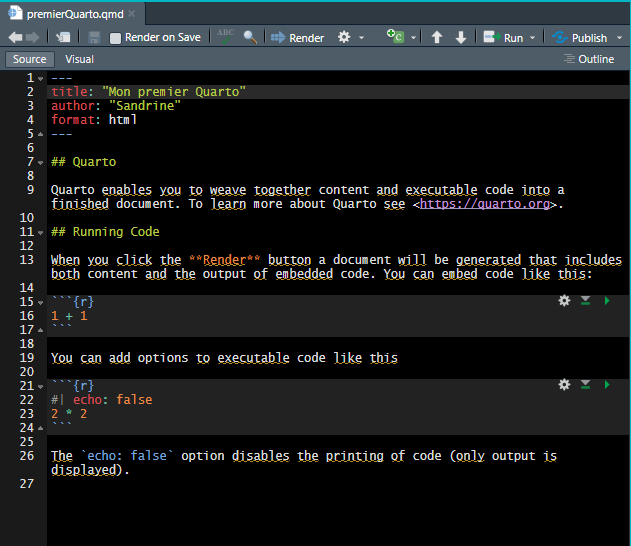
\includegraphics[width=0.75\linewidth,height=\textheight,keepaspectratio]{img/premierQuarto.png}
\end{center}

\begin{center}\rule{0.5\linewidth}{0.5pt}\end{center}

\subsubsection{3. Compiler (rendre) un
document}\label{compiler-rendre-un-document}

\begin{enumerate}
\def\labelenumi{\arabic{enumi}.}
\tightlist
\item
  Ouvrir le fichier \texttt{.qmd} créé dans \textbf{RStudio}\\
\item
  Modifier le titre dans le \textbf{YAML}\\
\item
  Cliquer sur \textbf{Render}\\
\item
  Consulter le résultat dans l'onglet \textbf{Viewer} ou dans le
  navigateur
\end{enumerate}


\includegraphics[width=1em,height=1em]{index_files/figure-pdf/fa-icon-a62d11e1500f8a927ee7cb35ace101f4.pdf}
Le bouton \textbf{Render} exécute le document

\begin{itemize}
\tightlist
\item
  il lance le code \textbf{R}\\
\item
  il insère les résultats\\
\item
  et il produit le fichier de sortie choisi
\end{itemize}

\subsection{\texorpdfstring{Le fichier
\texttt{.qmd}}{Le fichier .qmd}}\label{le-fichier-.qmd}

Un document \textbf{Quarto} contient généralement trois types de contenu

\begin{itemize}
\tightlist
\item
  \textbf{Des métadonnées} : titre, format, options\\
\item
  \textbf{Du texte} : titres, paragraphes, listes, liens\\
\item
  \textbf{Du code} : blocs \textbf{R} exécutés à la compilation (au
  rendu)
\end{itemize}


\includegraphics[width=0.75em,height=1em]{index_files/figure-pdf/fa-icon-04c6f9870c69c7270c705a206c46d917.pdf}
\textbf{L'extension \texttt{.qmd} signifie ``Quarto Markdown''}

\begin{center}\rule{0.5\linewidth}{0.5pt}\end{center}

\subsubsection{Exemple}\label{exemple}

\paragraph{Script Quarto (.qmd)}\label{script-quarto-.qmd}

\begin{center}
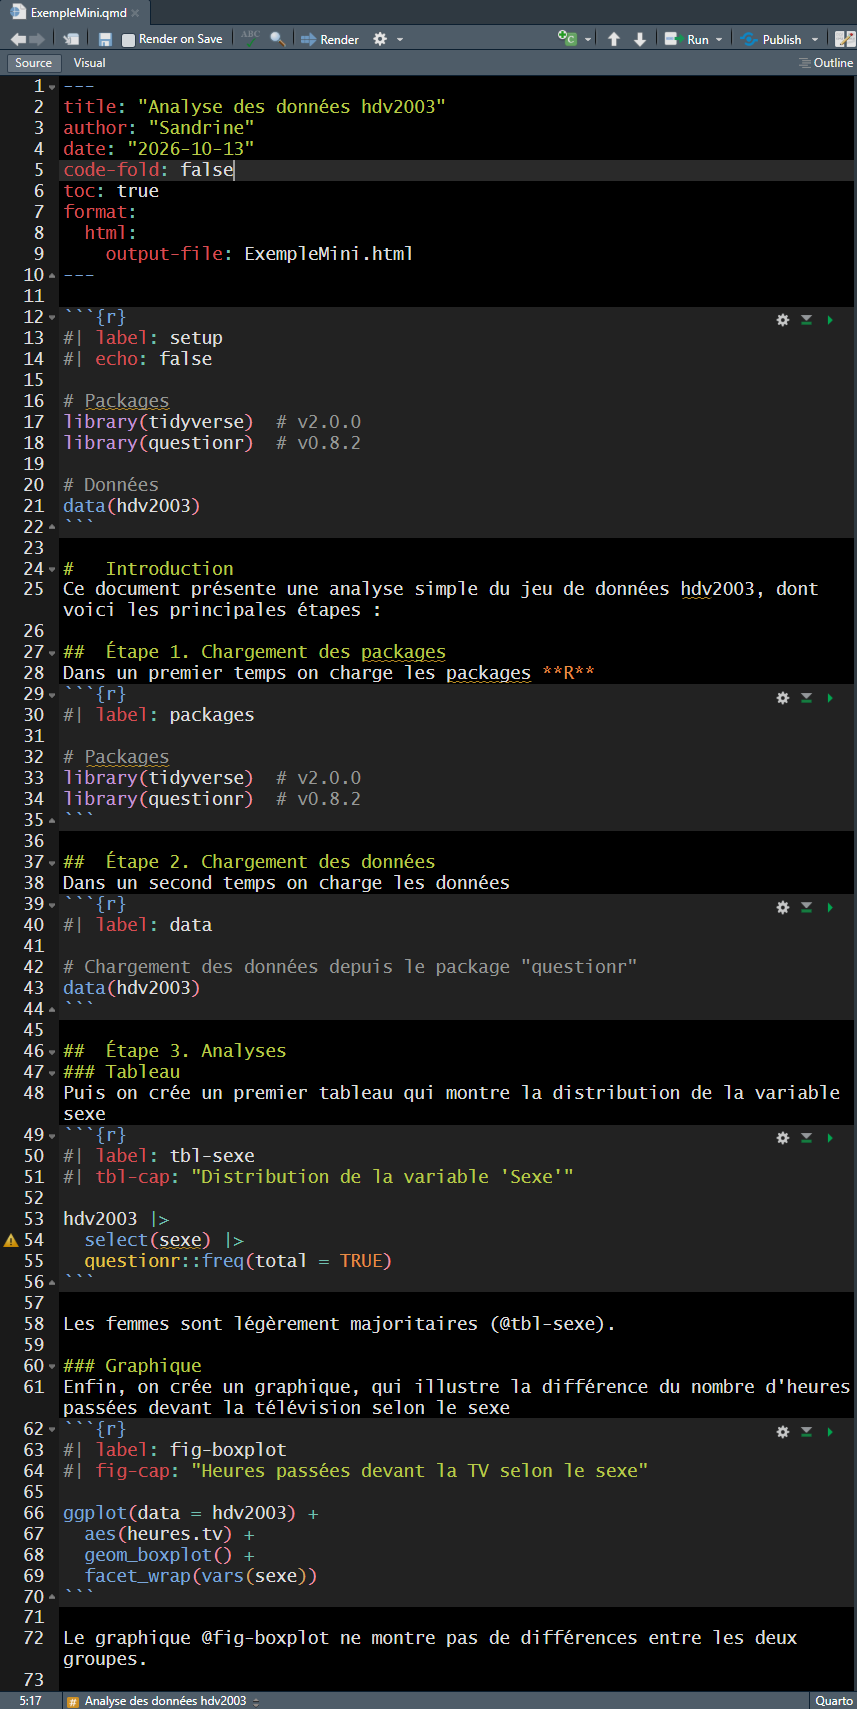
\includegraphics[width=2.86in,height=\textheight,keepaspectratio]{./img/qmd-script-example.png}
\end{center}


\includegraphics[width=1em,height=1em]{index_files/figure-pdf/fa-icon-dab55d07644b9a0a440f06723a45bcf5.pdf}

\paragraph{Rendu en html}\label{rendu-en-html}

\begin{center}
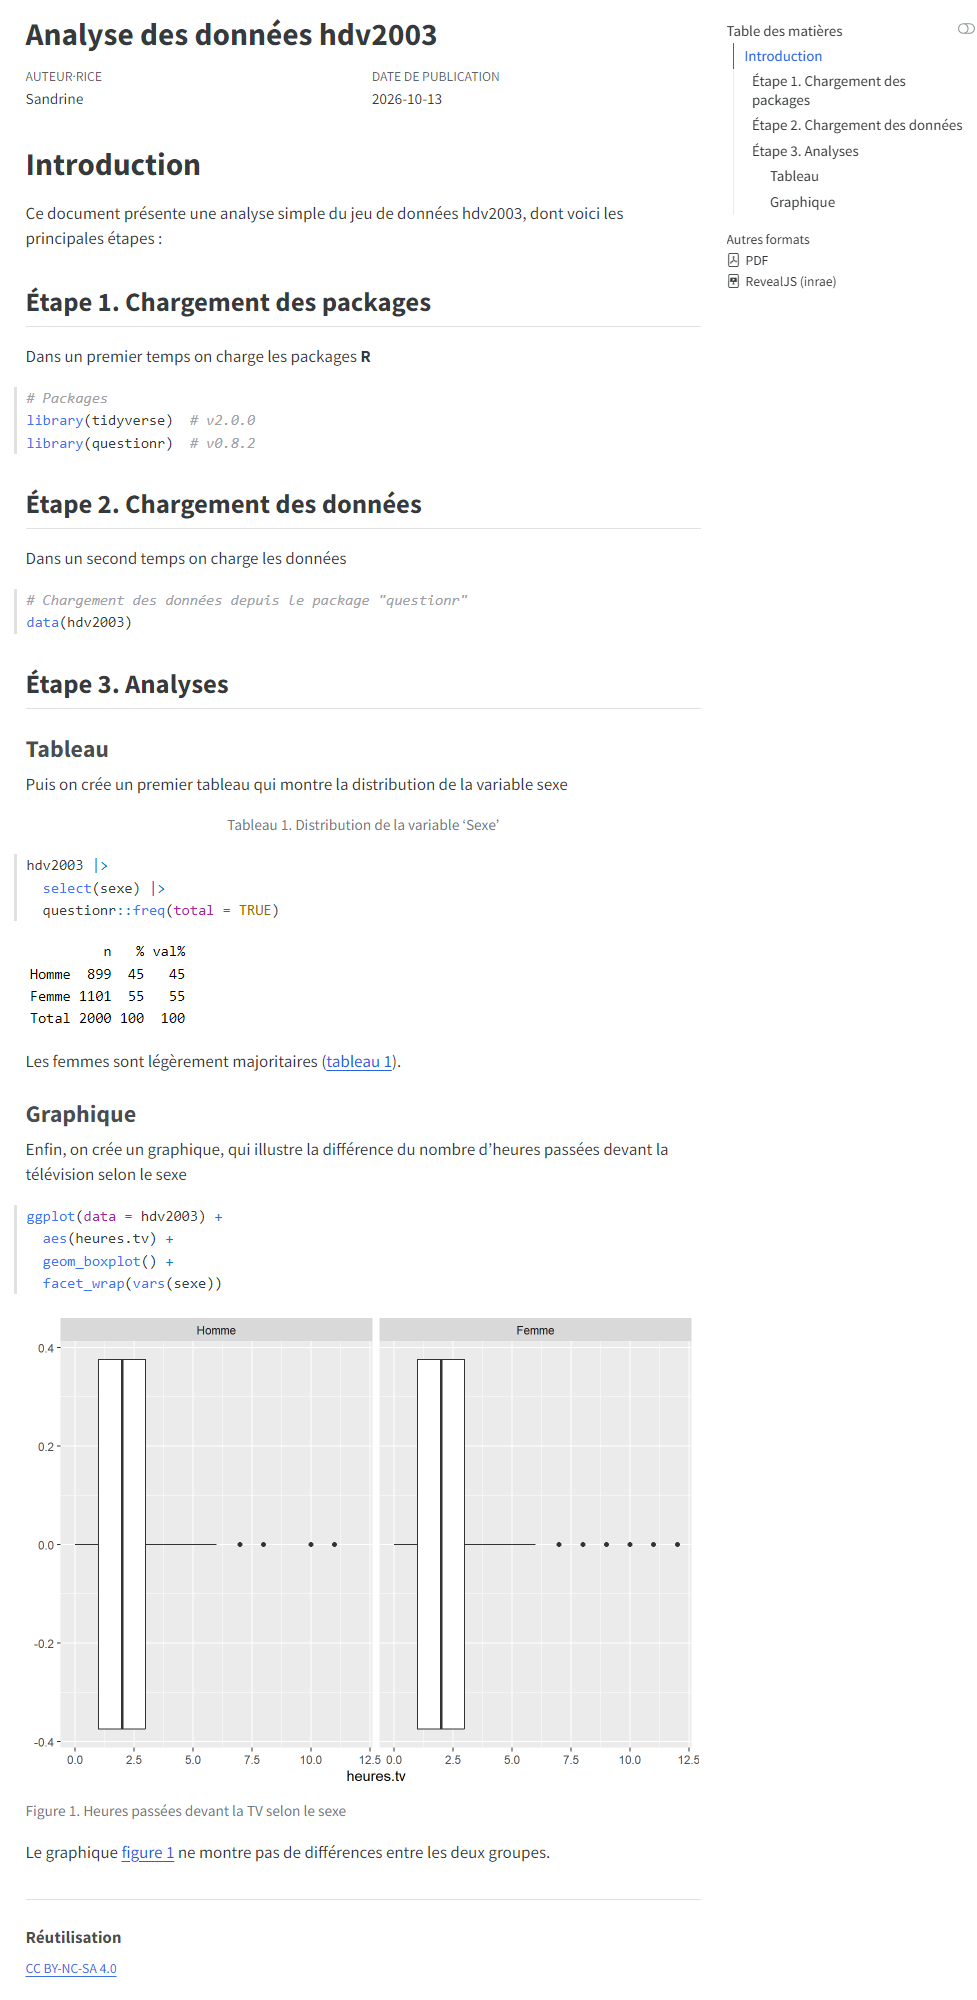
\includegraphics[width=3.26in,height=\textheight,keepaspectratio]{img/qmd-report-example.png}
\end{center}

\section{Utiliser Quarto}\label{utiliser-quarto}

\subsection{Écrire simplement avec
Markdown}\label{uxe9crire-simplement-avec-markdown}

\begin{itemize}
\tightlist
\item
  L'écriture sous \textbf{Quarto} s'appuie sur la syntaxe
  \textbf{Markdown}\\
  
\includegraphics[width=1em,height=1em]{index_files/figure-pdf/fa-icon-a978eb57bd05d19791fd4e4b9d979961.pdf}
  Les marqueurs \textbf{Markdown} sont des conventions simples que
  \textbf{Quarto} transforme à l'affichage\\
  
\includegraphics[width=1em,height=1em]{index_files/figure-pdf/fa-icon-be1da9f9a11cb30d6d0a10a027b462cd.pdf}
  \href{https://quarto.org/docs/authoring/markdown-basics.html}{Les
  bases en \textbf{Markdown}}\\
\item
  On peut écrire du code, des listes, des tableaux, des liens vers des
  pages web, des images, etc.\\
\item
  Il est également possible de gérer les
  \href{https://quarto.org/docs/authoring/citations.html}{citations} et
  les
  \href{https://quarto.org/docs/authoring/cross-references.html}{références
  croisées}
\end{itemize}

\emph{Exemple}

\begin{Shaded}
\begin{Highlighting}[]
\FunctionTok{\#\# Une diapositive}

\NormalTok{Un paragraphe explicatif}

\SpecialStringTok{{-} }\NormalTok{Premier point}
\SpecialStringTok{{-} }\NormalTok{Deuxième point}

\NormalTok{**Texte en gras** et *texte en italique*}
\end{Highlighting}
\end{Shaded}


\includegraphics[width=1em,height=1em]{index_files/figure-pdf/fa-icon-a62d11e1500f8a927ee7cb35ace101f4.pdf}
\textbf{Quarto} reprend les principes de \textbf{RMarkdown} mais
constitue un système plus général, compatible avec plusieurs langages de
programmation (\textbf{R}, \textbf{Python}, \textbf{Julia},
\textbf{JavaScript})

\begin{center}\rule{0.5\linewidth}{0.5pt}\end{center}

\subsubsection{\texorpdfstring{Syntaxe
\href{https://www.markdownguide.org/}{\textbf{Markdown}} pour la mise en
forme du
texte}{Syntaxe Markdown pour la mise en forme du texte}}\label{syntaxe-markdown-pour-la-mise-en-forme-du-texte}

{\def\LTcaptype{none} % do not increment counter
\begin{longtable}[]{@{}
  >{\raggedright\arraybackslash}p{(\linewidth - 4\tabcolsep) * \real{0.1789}}
  >{\raggedright\arraybackslash}p{(\linewidth - 4\tabcolsep) * \real{0.4000}}
  >{\raggedright\arraybackslash}p{(\linewidth - 4\tabcolsep) * \real{0.4211}}@{}}
\toprule\noalign{}
\begin{minipage}[b]{\linewidth}\raggedright
Caractéristique
\end{minipage} & \begin{minipage}[b]{\linewidth}\raggedright
Syntaxe Markdown
\end{minipage} & \begin{minipage}[b]{\linewidth}\raggedright
Résultat
\end{minipage} \\
\midrule\noalign{}
\endhead
\bottomrule\noalign{}
\endlastfoot
italic & \texttt{texte\ en\ *italique*} & texte en \emph{italique} \\
bold & \texttt{texte\ en\ **gras**} & texte en \textbf{gras} \\
superscript & \texttt{superficie\ de\ 200\ m\^{}2\^{}} & superficie de
200 m\textsuperscript{2} \\
subscript &
\texttt{Les\ individus\ notés\ n\textasciitilde{}i\textasciitilde{}} &
Les individus notés n\textsubscript{i} \\
headings & \texttt{\#\ Titre\ 1} & \# Titre 1 \\
& \texttt{\#\#\ Titre\ 2} & \#\# Titre 2 \\
& \texttt{\#\#\#\ Titre\ 3} & \#\#\# Titre 3 \\
& \texttt{\#\#\#\#\ Titre\ 4} & \#\#\#\# Titre 4 \\
& \texttt{\#\#\#\#\#\ Titre\ 5} & \#\#\#\#\# Titre 5 \\
& \texttt{\#\#\#\#\#\#\ Titre\ 6} & \#\#\#\#\#\# Titre 6 \\
links & Site \texttt{{[}Quarto{]}(https://quarto.org/)} & Site
\href{https://quarto.org/}{\textbf{Quarto}} \\
visible links & le lien est
\texttt{\textless{}https://quarto.org/\textgreater{}} & le lien est
\url{https://quarto.org} \\
\end{longtable}
}


\includegraphics[width=0.75em,height=1em]{index_files/figure-pdf/fa-icon-04c6f9870c69c7270c705a206c46d917.pdf}
\textbf{Il n'est pas possible de souligner du texte en Markdown}, le
soulignement étant réservé aux liens hypertextes

\subsection{Le YAML}\label{le-yaml}

\subsubsection{Définir les paramètres du document et du
rendu}\label{duxe9finir-les-paramuxe8tres-du-document-et-du-rendu}

\begin{itemize}
\tightlist
\item
  Dans un fichier \texttt{.qmd}, le bloc YAML se trouve généralement au
  début du document, entre deux lignes de trois tirets
  \texttt{-\/-\/-}\\
\item
  Il donne à \textbf{Quarto} des informations sur le document et indique
  le format de sortie

  \begin{itemize}
  \tightlist
  \item
    les métadonnées : titre, auteur, date, langue, etc.\\
  \item
    les options sur les formats de sortie : \texttt{html}, \texttt{pdf},
    \texttt{word}, \texttt{revealjs}, etc.
  \item
    les options de mise en page : table des matières, apparence, etc.
  \end{itemize}
\end{itemize}

\begin{Shaded}
\begin{Highlighting}[]
\PreprocessorTok{{-}{-}{-}}
\FunctionTok{title}\KeywordTok{:}\AttributeTok{ }\StringTok{"Découvrir Quarto sous R"}
\FunctionTok{author}\KeywordTok{:}\AttributeTok{ }\StringTok{"Nom et prénom"}
\FunctionTok{date}\KeywordTok{:}\AttributeTok{ }\StringTok{"2026{-}10{-}13"}
\FunctionTok{lang}\KeywordTok{:}\AttributeTok{ fr}
\FunctionTok{format}\KeywordTok{:}
\AttributeTok{  }\FunctionTok{revealjs}\KeywordTok{:}
\AttributeTok{    }\FunctionTok{theme}\KeywordTok{:}\AttributeTok{ simple}
\AttributeTok{    }\FunctionTok{slide{-}number}\KeywordTok{:}\AttributeTok{ }\CharTok{true}
\PreprocessorTok{{-}{-}{-}}
\end{Highlighting}
\end{Shaded}


\includegraphics[width=1em,height=1em]{index_files/figure-pdf/fa-icon-09adc4e6f7e3a3ea6746cbc6d7cc075a.pdf}
\textbf{Le YAML est le premier élément évalué lors de la compilation}\\

\includegraphics[width=1em,height=1em]{index_files/figure-pdf/fa-icon-a978eb57bd05d19791fd4e4b9d979961.pdf}
En cas d'erreur, la compilation s'arrête quasi instantanément

\begin{center}\rule{0.5\linewidth}{0.5pt}\end{center}

\subsubsection{Écrire le YAML}\label{uxe9crire-le-yaml}

\begin{itemize}
\tightlist
\item
  \texttt{title} : le titre du document
\item
  \texttt{author} : le nom de l'auteur ou de l'autrice
\item
  \texttt{date} : la date affichée
\item
  \texttt{lang} : la langue du document, ici le français
\item
  \texttt{format} : le type de sortie demandé
\item
  \texttt{revealjs} : des diapositives \texttt{html} avec
  \texttt{revealjs}
\item
  \texttt{theme} et \texttt{slide-number} : des options de présentation
\end{itemize}


\includegraphics[width=1em,height=1em]{index_files/figure-pdf/fa-icon-09adc4e6f7e3a3ea6746cbc6d7cc075a.pdf}
\textbf{La syntaxe est très sensible à l'indentation}\\

\includegraphics[width=1em,height=1em]{index_files/figure-pdf/fa-icon-a978eb57bd05d19791fd4e4b9d979961.pdf}
\textbf{Ajouter 2 espaces pour chaque niveau d'indentation}

\emph{Dans l'exemple précédent, les options placées sous
\texttt{revealjs} appartiennent à ce format}

\begin{tcolorbox}[enhanced jigsaw, arc=.35mm, bottomrule=.15mm, breakable, colback=white, colframe=quarto-callout-note-color-frame, left=2mm, leftrule=.75mm, opacityback=0, rightrule=.15mm, toprule=.15mm]
\begin{minipage}[t]{5.5mm}
\textcolor{quarto-callout-note-color}{\faInfo}
\end{minipage}%
\begin{minipage}[t]{\textwidth - 5.5mm}

\vspace{-3mm}\textbf{Voir la documentation Quarto pour plus d'informations sur les nombreuses
options disponibles}\vspace{3mm}

\begin{itemize}
\tightlist
\item
  section
  \href{https://quarto.org/docs/authoring/front-matter.html}{Front
  matter}\\
\item
  pour le format
  \href{https://quarto.org/docs/reference/formats/html.html}{HTML}\\
\item
  pour le format
  \href{https://quarto.org/docs/reference/formats/pdf.html}{PDF}\\
\item
  pour le format
  \href{https://quarto.org/docs/reference/formats/docx.html}{Word}\\
\item
  pour le format
  \href{https://quarto.org/docs/reference/formats/presentations/revealjs.html}{Revealjs}\\
\item
  pour le format
  \href{https://quarto.org/docs/reference/formats/presentations/pptx.html}{Powerpoint}\\
\end{itemize}

\end{minipage}%
\end{tcolorbox}

\begin{center}\rule{0.5\linewidth}{0.5pt}\end{center}

\subsubsection{Personnaliser les rendus}\label{personnaliser-les-rendus}

Le YAML permet de régler le thème et le numéro des diapositives, ou
encore la création d'une table des matières ou l'utilisation d'une base
bibliographique (au format \texttt{.bib})

\begin{Shaded}
\begin{Highlighting}[]
\FunctionTok{format}\KeywordTok{:}
\AttributeTok{  }\FunctionTok{revealjs}\KeywordTok{:}
\AttributeTok{    }\FunctionTok{theme}\KeywordTok{:}\AttributeTok{ simple}
\AttributeTok{    }\FunctionTok{slide{-}number}\KeywordTok{:}\AttributeTok{ }\CharTok{true}
\AttributeTok{  }\FunctionTok{pdf}\KeywordTok{:}\AttributeTok{ }
\AttributeTok{    }\FunctionTok{toc}\KeywordTok{:}\AttributeTok{ }\CharTok{true}
\FunctionTok{bibliography}\KeywordTok{:}\AttributeTok{ mon\_fichier.bib}
\end{Highlighting}
\end{Shaded}


\includegraphics[width=0.75em,height=1em]{index_files/figure-pdf/fa-icon-04c6f9870c69c7270c705a206c46d917.pdf}
Les thèmes prédéfinis incluent notamment \texttt{simple}, \texttt{dark},
\texttt{solarized} et \texttt{beige}. Il est possible de créer son
propre thème en le personnalisant avec le \texttt{css}


\includegraphics[width=1em,height=1em]{index_files/figure-pdf/fa-icon-09adc4e6f7e3a3ea6746cbc6d7cc075a.pdf}
Mieux vaut commencer par quelques options utiles et ajouter le reste
selon les besoins

\begin{center}\rule{0.5\linewidth}{0.5pt}\end{center}

\subsubsection{Où placer les réglages YAML
?}\label{ouxf9-placer-les-ruxe9glages-yaml}

Les réglages \textbf{YAML} peuvent être spécifiés dans un fichier séparé
pour éviter

\begin{itemize}
\tightlist
\item
  de répéter dans chaque \texttt{.qmd} les options communes au projet\\
\item
  un long bloc \textbf{YAML} en début de script
\end{itemize}


\includegraphics[width=0.75em,height=1em]{index_files/figure-pdf/fa-icon-04c6f9870c69c7270c705a206c46d917.pdf}
\textbf{Règle pratique}

\begin{itemize}
\tightlist
\item
  les options communes dans \texttt{\_quarto.yml}\\
\item
  les spécificités dans le \texttt{.qmd}
\end{itemize}

{\def\LTcaptype{none} % do not increment counter
\begin{longtable}[]{@{}lll@{}}
\toprule\noalign{}
Niveau & Fichier & Portée \\
\midrule\noalign{}
\endhead
\bottomrule\noalign{}
\endlastfoot
Document & YAML en tête du \texttt{.qmd} & Ce document seulement \\
Dossier & \texttt{\_metadata.yml} & Documents du dossier \\
Projet & \texttt{\_quarto.yml} & Tous les documents du projet \\
\end{longtable}
}

\emph{Exemple}

\begin{Shaded}
\begin{Highlighting}[]
\CommentTok{\# \_quarto.yml}
\FunctionTok{project}\KeywordTok{:}
\AttributeTok{  }\FunctionTok{type}\KeywordTok{:}\AttributeTok{ default}

\FunctionTok{format}\KeywordTok{:}
\AttributeTok{  }\FunctionTok{revealjs}\KeywordTok{:}
\AttributeTok{    }\FunctionTok{theme}\KeywordTok{:}\AttributeTok{ simple}
\AttributeTok{    }\FunctionTok{slide{-}number}\KeywordTok{:}\AttributeTok{ }\CharTok{true}

\FunctionTok{execute}\KeywordTok{:}
\AttributeTok{  }\FunctionTok{echo}\KeywordTok{:}\AttributeTok{ }\CharTok{true}
\end{Highlighting}
\end{Shaded}

\subsection{Produire un rapport : Word ou
pdf}\label{produire-un-rapport-word-ou-pdf}


\includegraphics[width=0.75em,height=1em]{index_files/figure-pdf/fa-icon-04c6f9870c69c7270c705a206c46d917.pdf}
Le même fichier \texttt{.qmd} peut produire une page html, une
présentation, un document Word ou un pdf


\includegraphics[width=1em,height=1em]{index_files/figure-pdf/fa-icon-a978eb57bd05d19791fd4e4b9d979961.pdf}
\textbf{Bonne pratique :} rédiger et maintenir le \texttt{.qmd}, puis
générer le format selon les besoins

\emph{Exemple}

\begin{Shaded}
\begin{Highlighting}[]
\PreprocessorTok{{-}{-}{-}}
\FunctionTok{title}\KeywordTok{:}\AttributeTok{ }\StringTok{"Rapport d\textquotesingle{}analyse"}
\FunctionTok{author}\KeywordTok{:}\AttributeTok{ }\StringTok{"Nom et prénom"}
\FunctionTok{date}\KeywordTok{:}\AttributeTok{ today}
\FunctionTok{lang}\KeywordTok{:}\AttributeTok{ fr}
\FunctionTok{format}\KeywordTok{:}
\AttributeTok{  }\FunctionTok{docx}\KeywordTok{:}
\AttributeTok{    }\FunctionTok{toc}\KeywordTok{:}\AttributeTok{ }\CharTok{true}
\AttributeTok{  }\FunctionTok{pdf}\KeywordTok{:}
\AttributeTok{    }\FunctionTok{toc}\KeywordTok{:}\AttributeTok{ }\CharTok{true}
\AttributeTok{    }\FunctionTok{number{-}sections}\KeywordTok{:}\AttributeTok{ }\CharTok{true}
\PreprocessorTok{{-}{-}{-}}
\end{Highlighting}
\end{Shaded}

\textbf{Comment lire ce YAML?}

\begin{itemize}
\tightlist
\item
  \texttt{docx} produit un fichier Word modifiable\\
\item
  \texttt{pdf} produit un document pdf non modifiable
\item
  \texttt{toc:\ true} ajoute une table des matières au document\\
\item
  \texttt{number-sections:\ true} numérote les sections dans le pdf\\
\end{itemize}


\includegraphics[width=1.25em,height=1em]{index_files/figure-pdf/fa-icon-f6ab0958e2b101a9fcd6422aa37dba7f.pdf}
\textbf{Commandes à exécuter dans un terminal, pour obtenir le rendu
dans un format précis}

\begin{Shaded}
\begin{Highlighting}[]
\ExtensionTok{quarto}\NormalTok{ render rapport.qmd }\AttributeTok{{-}{-}to}\NormalTok{ docx}
\ExtensionTok{quarto}\NormalTok{ render rapport.qmd }\AttributeTok{{-}{-}to}\NormalTok{ pdf}
\end{Highlighting}
\end{Shaded}


\includegraphics[width=1em,height=1em]{index_files/figure-pdf/fa-icon-dfa8ddbdb4ee1ddd96608f1a2bb8f38a.pdf}
Le rendu PDF nécessite généralement une distribution \textbf{LaTeX}, par
exemple \textbf{TinyTeX}, pensez à vérifier que c'est installé sur votre
machine

\subsection{Créer une diapositive}\label{cruxe9er-une-diapositive}

Avec \texttt{revealjs}, 2 balises \texttt{\#} successives
(\texttt{\#\#}) créent les diapositives

\begin{Shaded}
\begin{Highlighting}[]
\FunctionTok{\#\# Première diapositive}

\NormalTok{Contenu de la première diapositive}

\FunctionTok{\#\# Deuxième diapositive}

\NormalTok{Contenu de la deuxième diapositive}
\end{Highlighting}
\end{Shaded}


\includegraphics[width=0.75em,height=1em]{index_files/figure-pdf/fa-icon-04c6f9870c69c7270c705a206c46d917.pdf}
Une seule balise \texttt{\#} sert à créer des sections avec une
diapositive de titre

\subsection{Ajouter un bloc de code R}\label{ajouter-un-bloc-de-code-r}

\begin{itemize}
\tightlist
\item
  Un bloc \textbf{R} exécutable commence par
  \texttt{\textasciigrave{}\textasciigrave{}\textasciigrave{}\{r\}} et
  se termine par trois accents graves (\emph{back ticks})\\
\item
  Dans le rendu, \textbf{Quarto} peut inclure le code, le résultat, ou
  les deux selon les options choisies\\
\item
  Les options commencent par le \emph{hashpipe} \texttt{\#\textbar{}} et
  s'écrivent en utilisant la syntaxe : \texttt{option:\ value}
\end{itemize}

\begin{Shaded}
\begin{Highlighting}[]
\InformationTok{\textasciigrave{}\textasciigrave{}\textasciigrave{}\{r\}}
\CommentTok{\# Distribution de la variable "age"}
\NormalTok{hdv2003 }\SpecialCharTok{|\textgreater{}} 
  \FunctionTok{select}\NormalTok{(age) }\SpecialCharTok{|\textgreater{}} 
  \FunctionTok{summary}\NormalTok{()}
\InformationTok{\textasciigrave{}\textasciigrave{}\textasciigrave{}}
\end{Highlighting}
\end{Shaded}

\begin{verbatim}
      age       
 Min.   :18.00  
 1st Qu.:35.00  
 Median :48.00  
 Mean   :48.16  
 3rd Qu.:60.00  
 Max.   :97.00  
\end{verbatim}


\includegraphics[width=0.75em,height=1em]{index_files/figure-pdf/fa-icon-04c6f9870c69c7270c705a206c46d917.pdf}
Dans cet exemple, le code et le résultat sont affichés car le bloc de
code est écrit avec les options

\begin{itemize}
\tightlist
\item
  \texttt{\#\textbar{}\ echo:\ true} pour afficher le code\\
\item
  \texttt{\#\textbar{}\ eval:\ true} pour afficher le résultat\\
\end{itemize}

\begin{tcolorbox}[enhanced jigsaw, arc=.35mm, bottomrule=.15mm, breakable, colback=white, colframe=quarto-callout-tip-color-frame, left=2mm, leftrule=.75mm, opacityback=0, rightrule=.15mm, toprule=.15mm]

\begin{itemize}
\item
  \textbf{R n'est pas le seul langage possible dans les blocs de code}\\
  
\includegraphics[width=1em,height=1em]{index_files/figure-pdf/fa-icon-a978eb57bd05d19791fd4e4b9d979961.pdf}
  On spécifie le langage souhaité dans les accolades \{\} sur la
  première ligne du bloc de code, à la suite des ```\\
\item
  \textbf{Pour afficher directement le résultat d'un calcul dans une
  phrase, on insère directement le code dans la phrase, en utilisant un
  seul \emph{back tick} ` pour encadrer le code}

  \begin{itemize}
  \tightlist
  \item
    \textbf{Syntaxe} : L'âge moyen des
    `\texttt{\{r\}\ hdv2003\ \textbar{}\textgreater{}\ nrow()}`
    observations de hdv2003 est égal à
    `\texttt{\{r\}\ hdv2003\ \textbar{}\textgreater{}\ pull(age)\ \textbar{}\textgreater{}\ mean(na.rm\ =\ TRUE)}`\\
  \item
    \textbf{Résultat} : L'âge moyen des 2000 observations de hdv2003 est
    égal à 48.157
  \end{itemize}
\end{itemize}

\end{tcolorbox}

\begin{center}\rule{0.5\linewidth}{0.5pt}\end{center}

\subsubsection{Paramétrer les blocs de
code}\label{paramuxe9trer-les-blocs-de-code}

Les options des blocs de code s'écrivent avec le préfixe
\texttt{\#\textbar{}} et permettent de contrôler l'exécution,
l'affichage du code et la mise en forme des sorties

\begin{longtable}[]{@{}
  >{\raggedright\arraybackslash}p{(\linewidth - 2\tabcolsep) * \real{0.2537}}
  >{\raggedright\arraybackslash}p{(\linewidth - 2\tabcolsep) * \real{0.7463}}@{}}
\caption{Principales options des blocs de code}\tabularnewline
\toprule\noalign{}
\begin{minipage}[b]{\linewidth}\raggedright
Option
\end{minipage} & \begin{minipage}[b]{\linewidth}\raggedright
Description
\end{minipage} \\
\midrule\noalign{}
\endfirsthead
\toprule\noalign{}
\begin{minipage}[b]{\linewidth}\raggedright
Option
\end{minipage} & \begin{minipage}[b]{\linewidth}\raggedright
Description
\end{minipage} \\
\midrule\noalign{}
\endhead
\bottomrule\noalign{}
\endlastfoot
\texttt{label} & Donner un nom au bloc (utile pour le référencer et y
faire appel dans le texte) \\
\texttt{eval:\ true/false} & Exécuter le code du bloc \\
\texttt{echo:\ true/false} & Afficher le code dans le document final \\
\texttt{include:\ true/false} & Contrôler l'inclusion du code et/ou des
résultats dans le document final (\texttt{false} : supprime tout) \\
\texttt{warning:\ true/false} & Inclure les avertissements générés dans
le document final \\
\texttt{message:\ true/false} & Afficher dans le document final, les
messages générés par le code \\
\end{longtable}

\begin{center}\rule{0.5\linewidth}{0.5pt}\end{center}

\subsubsection{Nommer les blocs de code}\label{nommer-les-blocs-de-code}

Chaque bloc de code peut recevoir un \textbf{label}

\begin{itemize}
\tightlist
\item
  qui doit être un nom composé de chiffres et de lettres, court,
  explicite et \textbf{unique} (les tirets \texttt{-} et les
  \emph{underscores} \texttt{\_} sont autorisés, en revanche les espaces
  et caractères spéciaux sont déconseillés)\\
\item
  doit être placé de préférence sur la première ligne du bloc de code,
  avant les autres options
\end{itemize}

\begin{Shaded}
\begin{Highlighting}[]
\InformationTok{\textasciigrave{}\textasciigrave{}\textasciigrave{}\{r\}}
\CommentTok{\#| label: datahdv}
\CommentTok{\#| eval: true}
\FunctionTok{data}\NormalTok{(hdv2003)}
\InformationTok{\textasciigrave{}\textasciigrave{}\textasciigrave{}}
\end{Highlighting}
\end{Shaded}


\includegraphics[width=0.75em,height=1em]{index_files/figure-pdf/fa-icon-04c6f9870c69c7270c705a206c46d917.pdf}
\textbf{Il permet d'identifier le bloc dans le document et dans les
messages d'erreur} et de faciliter la lecture et la maintenance d'un
document long

\begin{center}\rule{0.5\linewidth}{0.5pt}\end{center}

\subsubsection{Cas particulier des blocs de codes des tableaux et
figures}\label{cas-particulier-des-blocs-de-codes-des-tableaux-et-figures}

\paragraph{Référencer tableaux et figures dans le
texte}\label{ruxe9fuxe9rencer-tableaux-et-figures-dans-le-texte}

\begin{itemize}
\tightlist
\item
  On donne des noms de labels au bloc de code avec un préfixe spécifique
  : \texttt{tbl-} pour les tableaux ; \texttt{fig-} pour les figures
  (images, graphiques)
\item
  On peut donner une légende avec les options
  \texttt{\#\textbar{}\ tbl-cap:} pour les tableaux ;
  \texttt{\#\textbar{}\ fig-cap:} pour les figures
\item
  On fait ensuite référence au tableau ou à la figure avec
  \texttt{@prefixe-nom} dans le texte
\end{itemize}

\subparagraph{Bloc de code}\label{bloc-de-code}

\begin{Shaded}
\begin{Highlighting}[]
\CommentTok{\#| label: fig{-}sexeTV}
\CommentTok{\#| fig{-}height: 2}
\CommentTok{\#| fig{-}width: 3}
\CommentTok{\#| fig{-}cap: "Relation entre heures passées devant la TV et sexe des individus."}

\NormalTok{hdv2003 }\SpecialCharTok{|\textgreater{}} 
  \FunctionTok{ggplot}\NormalTok{() }\SpecialCharTok{+}
  \FunctionTok{aes}\NormalTok{(}\AttributeTok{x =}\NormalTok{ sexe, }\AttributeTok{y =}\NormalTok{ heures.tv) }\SpecialCharTok{+}
  \FunctionTok{geom\_boxplot}\NormalTok{()}
\end{Highlighting}
\end{Shaded}

\subparagraph{Résultat du bloc de
code}\label{ruxe9sultat-du-bloc-de-code}

\begin{figure}

\centering{

\pandocbounded{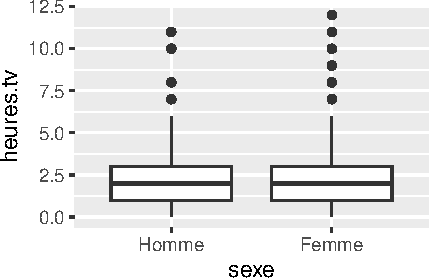
\includegraphics[keepaspectratio]{index_files/figure-pdf/fig-sexeTV-1.pdf}}

}

\caption{\label{fig-sexeTV}Relation entre heures passées devant la TV et
sexe des individus.}

\end{figure}%

\subparagraph{Référence dans le
texte}\label{ruxe9fuxe9rence-dans-le-texte}

\texttt{Comme\ illustré\ par\ la\ @fig-sexeTV,\ il\ y\ a\ peu\ de\ différences\ entre\ les\ groupes}

\subparagraph{Rendu}\label{rendu}

Comme illustré par la figure~\ref{fig-sexeTV}, il y a peu de différences
entre les groupes

\begin{center}\rule{0.5\linewidth}{0.5pt}\end{center}

\paragraph{Paramétrer le rendu des blocs de code des graphiques
R}\label{paramuxe9trer-le-rendu-des-blocs-de-code-des-graphiques-r}

Plusieurs options permettent d'améliorer le rendu des graphiques
\textbf{R}

{\def\LTcaptype{none} % do not increment counter
\begin{longtable}[]{@{}
  >{\raggedright\arraybackslash}p{(\linewidth - 4\tabcolsep) * \real{0.1386}}
  >{\raggedright\arraybackslash}p{(\linewidth - 4\tabcolsep) * \real{0.5149}}
  >{\raggedright\arraybackslash}p{(\linewidth - 4\tabcolsep) * \real{0.3465}}@{}}
\toprule\noalign{}
\begin{minipage}[b]{\linewidth}\raggedright
Option
\end{minipage} & \begin{minipage}[b]{\linewidth}\raggedright
Rôle
\end{minipage} & \begin{minipage}[b]{\linewidth}\raggedright
Exemple
\end{minipage} \\
\midrule\noalign{}
\endhead
\bottomrule\noalign{}
\endlastfoot
\texttt{label} & Identifie le bloc et permet une référence croisée &
\texttt{\#\textbar{}\ label:\ fig-age} \\
\texttt{fig-cap} & Ajoute une légende à la figure &
\texttt{\#\textbar{}\ fig-cap:\ "Distribution\ de\ la\ variable\ \textquotesingle{}age\textquotesingle{}"} \\
\texttt{fig-width} & Définit la largeur, en pouces, de la figure &
\texttt{\#\textbar{}\ fig-width:\ 7} \\
\texttt{fig-height} & Définit la hauteur, en pouces, de la figure &
\texttt{\#\textbar{}\ fig-height:\ 4.5} \\
\texttt{fig-align} & Définit l'alignement horizontal (\texttt{left},
\texttt{center} ou \texttt{right}) &
\texttt{\#\textbar{}\ fig-align:\ center} \\
\texttt{fig-alt} & Ajoute un texte alternatif pour les personnes qui ne
peuvent pas voir la figure &
\texttt{\#\textbar{}\ fig-alt:\ "Diagramme\ en\ boîte\ des\ heures\ quotidiennes\ passées\ devant\ la\ télévision\ selon\ le\ sexe"} \\
\texttt{dpi} & Définit la résolution de l'image produite &
\texttt{\#\textbar{}\ dpi:\ 300} \\
\end{longtable}
}

\subsection{Ajouter des tableaux}\label{ajouter-des-tableaux}

Un tableau peut être écrit directement en \textbf{Markdown} ou produit
par \textbf{R}

\subsubsection{Produire un tableau
manuellement}\label{produire-un-tableau-manuellement}

\begin{itemize}
\item
  Les tableaux directement écrits en \textbf{Markdown} sont

  \begin{itemize}
  \tightlist
  \item
    adaptés aux petits tableaux fixes\\
  \item
    simples à rédiger et à modifier
  \end{itemize}
\item
  L'alignement dans les cellules est contrôlé avec les \texttt{:}\\
  
\includegraphics[width=1em,height=1em]{index_files/figure-pdf/fa-icon-be1da9f9a11cb30d6d0a10a027b462cd.pdf}
  Voir la \href{https://quarto.org/docs/authoring/tables.html}{page
  d'aide Quarto dédiée} pour les options disponibles
\end{itemize}


\includegraphics[width=1em,height=1em]{index_files/figure-pdf/fa-icon-e38a8e106ce63d9b034a2d9721635ca8.pdf}
Les valeurs ne sont pas recalculées lors du rendu

\textbf{Syntaxe}

\begin{Shaded}
\begin{Highlighting}[]
\PreprocessorTok{|}\NormalTok{ Colonne 1   }\PreprocessorTok{|}\NormalTok{ Colonne 2   }\PreprocessorTok{|}\NormalTok{ Colonne 3   }\PreprocessorTok{|}\NormalTok{ Colonne 4   }\PreprocessorTok{|}
\PreprocessorTok{|:{-}{-}{-}{-}{-}{-}{-}{-}{-}{-}{-}{-}|:{-}{-}{-}{-}{-}{-}{-}{-}{-}{-}{-}:|{-}{-}{-}{-}{-}{-}{-}{-}{-}{-}{-}{-}:| {-}{-}{-}{-}{-}{-}{-}{-}{-}{-}{-}} \PreprocessorTok{|}
\PreprocessorTok{|}\NormalTok{ Alignement  }\PreprocessorTok{|}\NormalTok{ Alignement  }\PreprocessorTok{|}\NormalTok{ Alignement  }\PreprocessorTok{|}\NormalTok{ Alignement  }\PreprocessorTok{|}
\PreprocessorTok{|}\NormalTok{ à gauche    }\PreprocessorTok{|}\NormalTok{ centré      }\PreprocessorTok{|}\NormalTok{ à droite    }\PreprocessorTok{|}\NormalTok{ par défaut  }\PreprocessorTok{|}
\NormalTok{: Titre du tableau.}
\end{Highlighting}
\end{Shaded}

\textbf{Résultat}

\begin{longtable}[]{@{}lcrl@{}}
\caption{Titre du tableau.}\tabularnewline
\toprule\noalign{}
Colonne 1 & Colonne 2 & Colonne 3 & Colonne 4 \\
\midrule\noalign{}
\endfirsthead
\toprule\noalign{}
Colonne 1 & Colonne 2 & Colonne 3 & Colonne 4 \\
\midrule\noalign{}
\endhead
\bottomrule\noalign{}
\endlastfoot
Alignement & Alignement & Alignement & Alignement \\
à gauche & centré & à droite & par défaut \\
\end{longtable}


\includegraphics[width=1em,height=1em]{index_files/figure-pdf/fa-icon-50384ea67447599603fc85e2dddce4e1.pdf}
\textbf{Vous ne savez pas comment écrire un tableau en Markdown ?}\\

\includegraphics[width=1em,height=1em]{index_files/figure-pdf/fa-icon-a978eb57bd05d19791fd4e4b9d979961.pdf}
Utilisez \href{https://www.tablesgenerator.com/markdown_tables}{l'outil
en ligne}

\begin{center}\rule{0.5\linewidth}{0.5pt}\end{center}

\subsubsection{Produire un tableau avec
R}\label{produire-un-tableau-avec-r}

\begin{itemize}
\tightlist
\item
  Les tableaux produits par un bloc de code \textbf{R}

  \begin{itemize}
  \tightlist
  \item
    sont recalculés à chaque rendu
  \item
    sont cohérents avec les données et le code
  \item
    peuvent être référencés dans le texte grâce au label \texttt{tbl-}
  \item
    peuvent être décrits par une légende avec l'option
    \texttt{\#\textbar{}\ tbl-cap:}
  \end{itemize}
\item
  Les tableaux sont rendus propres et lisibles grâce à la fonction
  \texttt{kable()} du package \{\texttt{knitr}\}
\end{itemize}

\begin{Shaded}
\begin{Highlighting}[]
\InformationTok{\textasciigrave{}\textasciigrave{}\textasciigrave{}\{r\}}
\CommentTok{\#| label: tbl{-}hdv}
\CommentTok{\#| tbl{-}cap: "Extrait des données hdv2003."}
\NormalTok{hdv2003 }\SpecialCharTok{|\textgreater{}} 
  \FunctionTok{select}\NormalTok{(id}\SpecialCharTok{:}\NormalTok{qualif) }\SpecialCharTok{|\textgreater{}} 
  \FunctionTok{slice}\NormalTok{(}\DecValTok{1}\SpecialCharTok{:}\DecValTok{2}\NormalTok{) }\SpecialCharTok{|\textgreater{}} 
\NormalTok{  knitr}\SpecialCharTok{::}\FunctionTok{kable}\NormalTok{()}
\InformationTok{\textasciigrave{}\textasciigrave{}\textasciigrave{}}
\end{Highlighting}
\end{Shaded}

{

\begin{longtable}[]{@{}
  >{\raggedleft\arraybackslash}p{(\linewidth - 12\tabcolsep) * \real{0.0286}}
  >{\raggedleft\arraybackslash}p{(\linewidth - 12\tabcolsep) * \real{0.0381}}
  >{\raggedright\arraybackslash}p{(\linewidth - 12\tabcolsep) * \real{0.0571}}
  >{\raggedright\arraybackslash}p{(\linewidth - 12\tabcolsep) * \real{0.5048}}
  >{\raggedleft\arraybackslash}p{(\linewidth - 12\tabcolsep) * \real{0.0857}}
  >{\raggedright\arraybackslash}p{(\linewidth - 12\tabcolsep) * \real{0.2095}}
  >{\raggedright\arraybackslash}p{(\linewidth - 12\tabcolsep) * \real{0.0762}}@{}}

\caption{\label{tbl-hdv}Extrait des données hdv2003.}

\tabularnewline

\toprule\noalign{}
\begin{minipage}[b]{\linewidth}\raggedleft
id
\end{minipage} & \begin{minipage}[b]{\linewidth}\raggedleft
age
\end{minipage} & \begin{minipage}[b]{\linewidth}\raggedright
sexe
\end{minipage} & \begin{minipage}[b]{\linewidth}\raggedright
nivetud
\end{minipage} & \begin{minipage}[b]{\linewidth}\raggedleft
poids
\end{minipage} & \begin{minipage}[b]{\linewidth}\raggedright
occup
\end{minipage} & \begin{minipage}[b]{\linewidth}\raggedright
qualif
\end{minipage} \\
\midrule\noalign{}
\endhead
\bottomrule\noalign{}
\endlastfoot
1 & 28 & Femme & Enseignement superieur y compris technique superieur &
2634.398 & Exerce une profession & Employe \\
2 & 23 & Femme & NA & 9738.396 & Etudiant, eleve & NA \\

\end{longtable}

}

\subsection{Ajouter une image}\label{ajouter-une-image}

Une image non générée directement dans un bloc de code \textbf{R} peut
être insérée directement en \textbf{Markdown} avec la syntaxe suivante\\
\texttt{!{[}Texte{]}(chemin/image.extension)}

\begin{itemize}
\tightlist
\item
  le texte écrit dans les crochets est la légende de l'image\\
\item
  le chemin indiqué dans les parenthèses est relatif au fichier
  \texttt{.qmd}\\
  
\includegraphics[width=0.75em,height=1em]{index_files/figure-pdf/fa-icon-04c6f9870c69c7270c705a206c46d917.pdf}
  \textbf{Prévoir dans le projet un dossier qui stocke les images, pour
  faciliter l'organisation} (par exemple, \texttt{img/} comme ici pour
  cette présentation)
\end{itemize}

\textbf{Syntaxe Markdown}\\
\texttt{!{[}Logo\ Quarto{]}(img/quarto.png)}

\textbf{Résultat}

\begin{figure}[H]

{\centering \pandocbounded{
\includegraphics[keepaspectratio]{img/quarto.png}}

}

\caption{Logo Quarto}

\end{figure}%

\subsection{Ajouter une équation}\label{ajouter-une-uxe9quation}

L'écriture d'équations mathématiques est possible avec la syntaxe
\textbf{LaTeX}

\begin{itemize}
\tightlist
\item
  en ligne en encadrant l'équation par \texttt{\$}
\item
  en ``bloc'', centré au milieu de la page, en encadrant l'équation par
  \texttt{\$\$}
\end{itemize}

\subsubsection{Équation au sein d'un
texte}\label{uxe9quation-au-sein-dun-texte}

\textbf{Syntaxe}

\begin{Shaded}
\begin{Highlighting}[]
\NormalTok{La célèbre équation d\textquotesingle{}Einstein est $E = mc\^{}2$.}
\end{Highlighting}
\end{Shaded}

\textbf{Résultat}\\
La célèbre équation d'Einstein est \(E = mc^2\).

\subsubsection{Équation en bloc}\label{uxe9quation-en-bloc}

\textbf{Syntaxe}

\begin{Shaded}
\begin{Highlighting}[]
\NormalTok{La célèbre équation d\textquotesingle{}Einstein est }

\NormalTok{$$}
\NormalTok{E = mc\^{}2}
\NormalTok{$$}
\end{Highlighting}
\end{Shaded}

\textbf{Résultat}\\
La célèbre équation d'Einstein est\\
\[
E = mc^2
\]

\section{À retenir}\label{uxe0-retenir}

\subsection{En résumé}\label{en-ruxe9sumuxe9}

Les différents éléments pour utiliser \textbf{Quarto} sous \textbf{R}

\begin{itemize}
\tightlist
\item
  \texttt{.qmd} : le fichier source \textbf{Quarto}\\
\item
  \textbf{YAML} : les métadonnées et réglages du document\\
\item
  \textbf{Markdown} : la structure et le texte\\
\item
  Blocs \textbf{R} : le code exécuté et ses résultats\\
\item
  \texttt{render} : la commande qui produit la présentation
\end{itemize}

\section{Ressources}\label{ressources}

\subsection{Pour aller plus loin}\label{pour-aller-plus-loin}

De nombreuses ressources en ligne


\includegraphics[width=1em,height=1em]{index_files/figure-pdf/fa-icon-be1da9f9a11cb30d6d0a10a027b462cd.pdf}
\href{https://www.markdowntutorial.com/fr/}{Tutoriel
\textbf{Markdown}}\\

\includegraphics[width=1em,height=1em]{index_files/figure-pdf/fa-icon-be1da9f9a11cb30d6d0a10a027b462cd.pdf}
\href{https://quarto.org/docs/get-started/hello/rstudio.html}{Tutoriel
\textbf{Quarto}}\\

\includegraphics[width=1em,height=1em]{index_files/figure-pdf/fa-icon-be1da9f9a11cb30d6d0a10a027b462cd.pdf}
\href{https://quarto.org/docs/presentations/}{Documentation Quarto :
présentations}\\

\includegraphics[width=1em,height=1em]{index_files/figure-pdf/fa-icon-be1da9f9a11cb30d6d0a10a027b462cd.pdf}
\href{https://quarto.org/docs/presentations/revealjs/}{Guide Quarto pour
Reveal.js}\\

\includegraphics[width=1em,height=1em]{index_files/figure-pdf/fa-icon-be1da9f9a11cb30d6d0a10a027b462cd.pdf}
\href{https://quarto.org/docs/computations/execution-options/}{Documentation
Quarto : options d'exécution}\\

\includegraphics[width=1em,height=1em]{index_files/figure-pdf/fa-icon-be1da9f9a11cb30d6d0a10a027b462cd.pdf}
\href{https://quarto.org/docs/projects/quarto-projects.html}{Documentation
Quarto : projets et \texttt{\_quarto.yml}}\\
et plus encore dans la

\includegraphics[width=1em,height=1em]{index_files/figure-pdf/fa-icon-be1da9f9a11cb30d6d0a10a027b462cd.pdf}
\href{https://quarto.org/}{documentation officielle \textbf{Quarto}}




\end{document}
